\documentclass[9pt,lineno]{elife}
\usepackage{fullpage,amsmath,url,cases}
\usepackage{natbib,longtable,graphicx,tikz}

%%%%%%%%%%%%%%%%%%%%%%%%%%%%%%%%%% figure and table %%%%%%%%%%%%%%%%%%%%%%%%%%%%%%%%%%
\usepackage{graphicx}
\graphicspath{{./figures/}}
\usepackage{subfig}

\begin{document}


\begin{figure}[htp]
  \centering{}
  \subfloat[][]{
    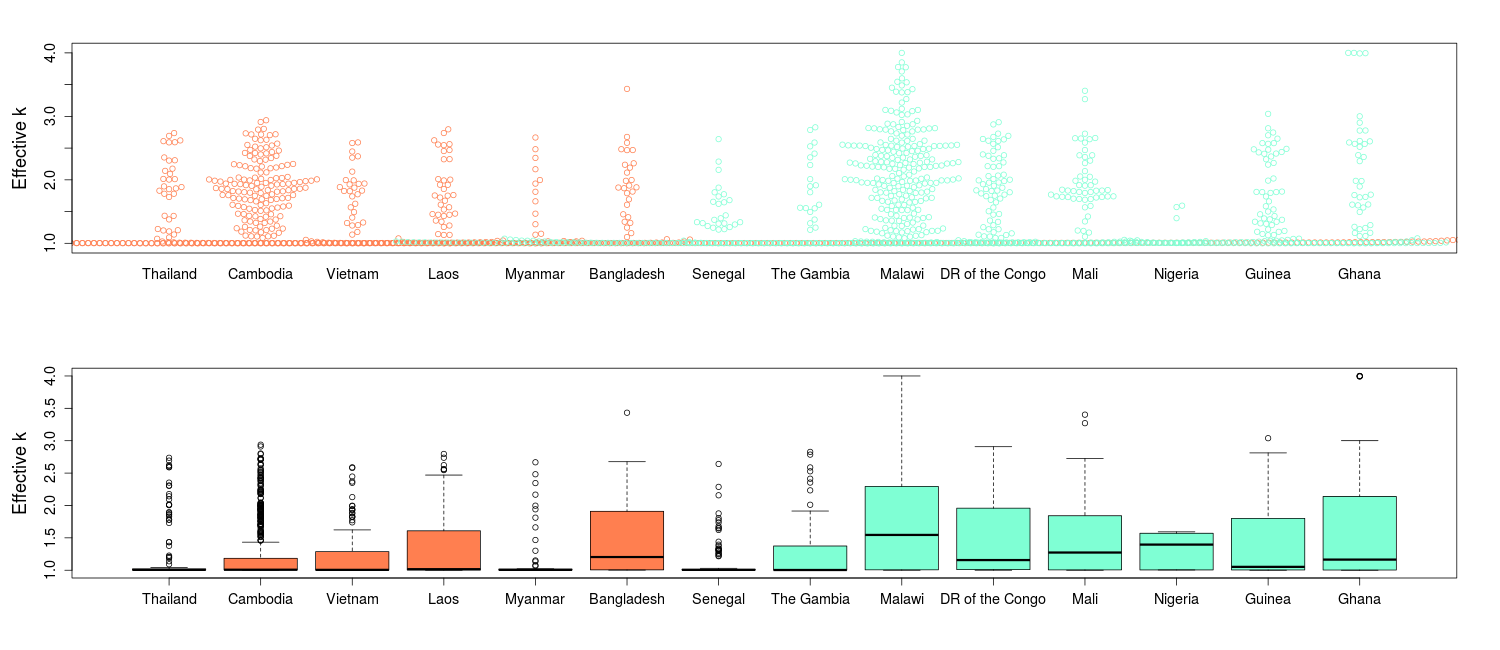
\includegraphics[width=0.7\textwidth]{beeswarm_effect_k.png}
  }\\
  \subfloat[][]{
  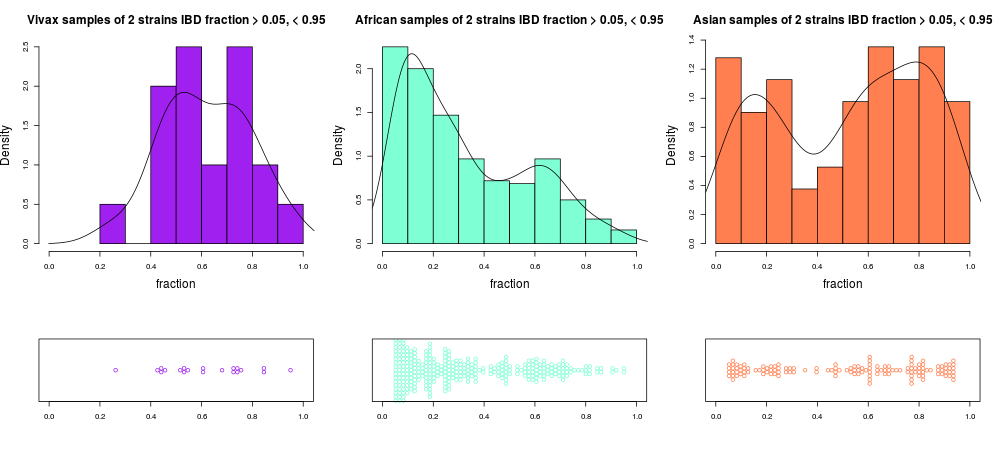
\includegraphics[width = 0.7\textwidth]{ibd_frac_hist.png}
  }\\
  \subfloat[][]{
    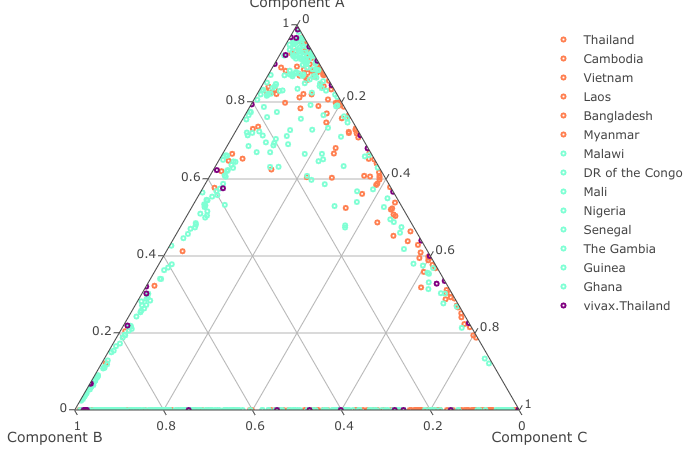
\includegraphics[width=0.7\textwidth]{ibdDistribution_withVivax.png}
  }\\
  %\subfloat[][]{
    %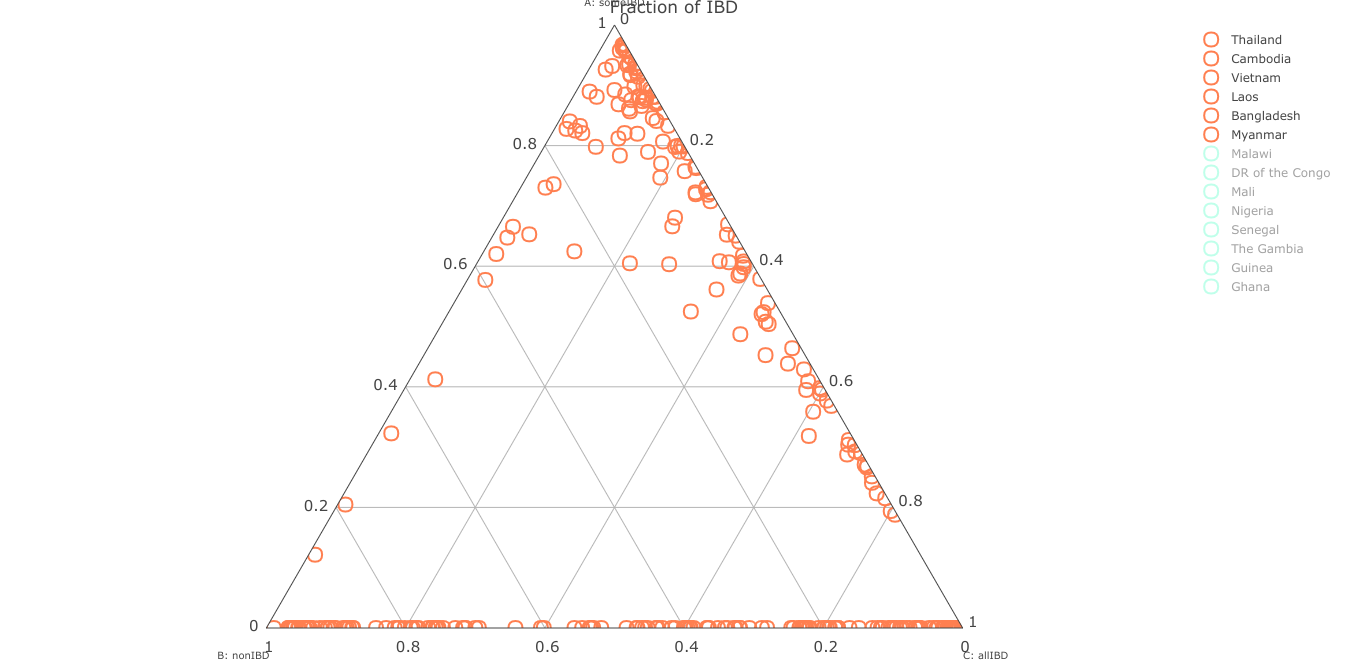
\includegraphics[width=0.8\textwidth]{ibdDistribution_asia.png}
  %}\\
  \caption{(a) Distribution of effective $k$ in each country. Countries in Asia show lower effective $k$ in Africa countries. Note Senegal and Gambia are similar to most Asia countries with low values of effective $k$. (b) Histograms of IBD fractions of two strain mixture samples. Relatedness structure of mixed samples peaks around 0.25, 0.5 suggest that mixed infections are caused by sib-strains. (c) Ternary plot of IBD fractions of all IBD, non-IBD and some-IBD of all mixed samples. Asia samples lean towards more IBD, Asia samples lean towards less IBD.}
  \label{fig:IBD_frac_hist}
\end{figure}

\begin{figure}[htp]
  \centering{}
  \subfloat[][]{
  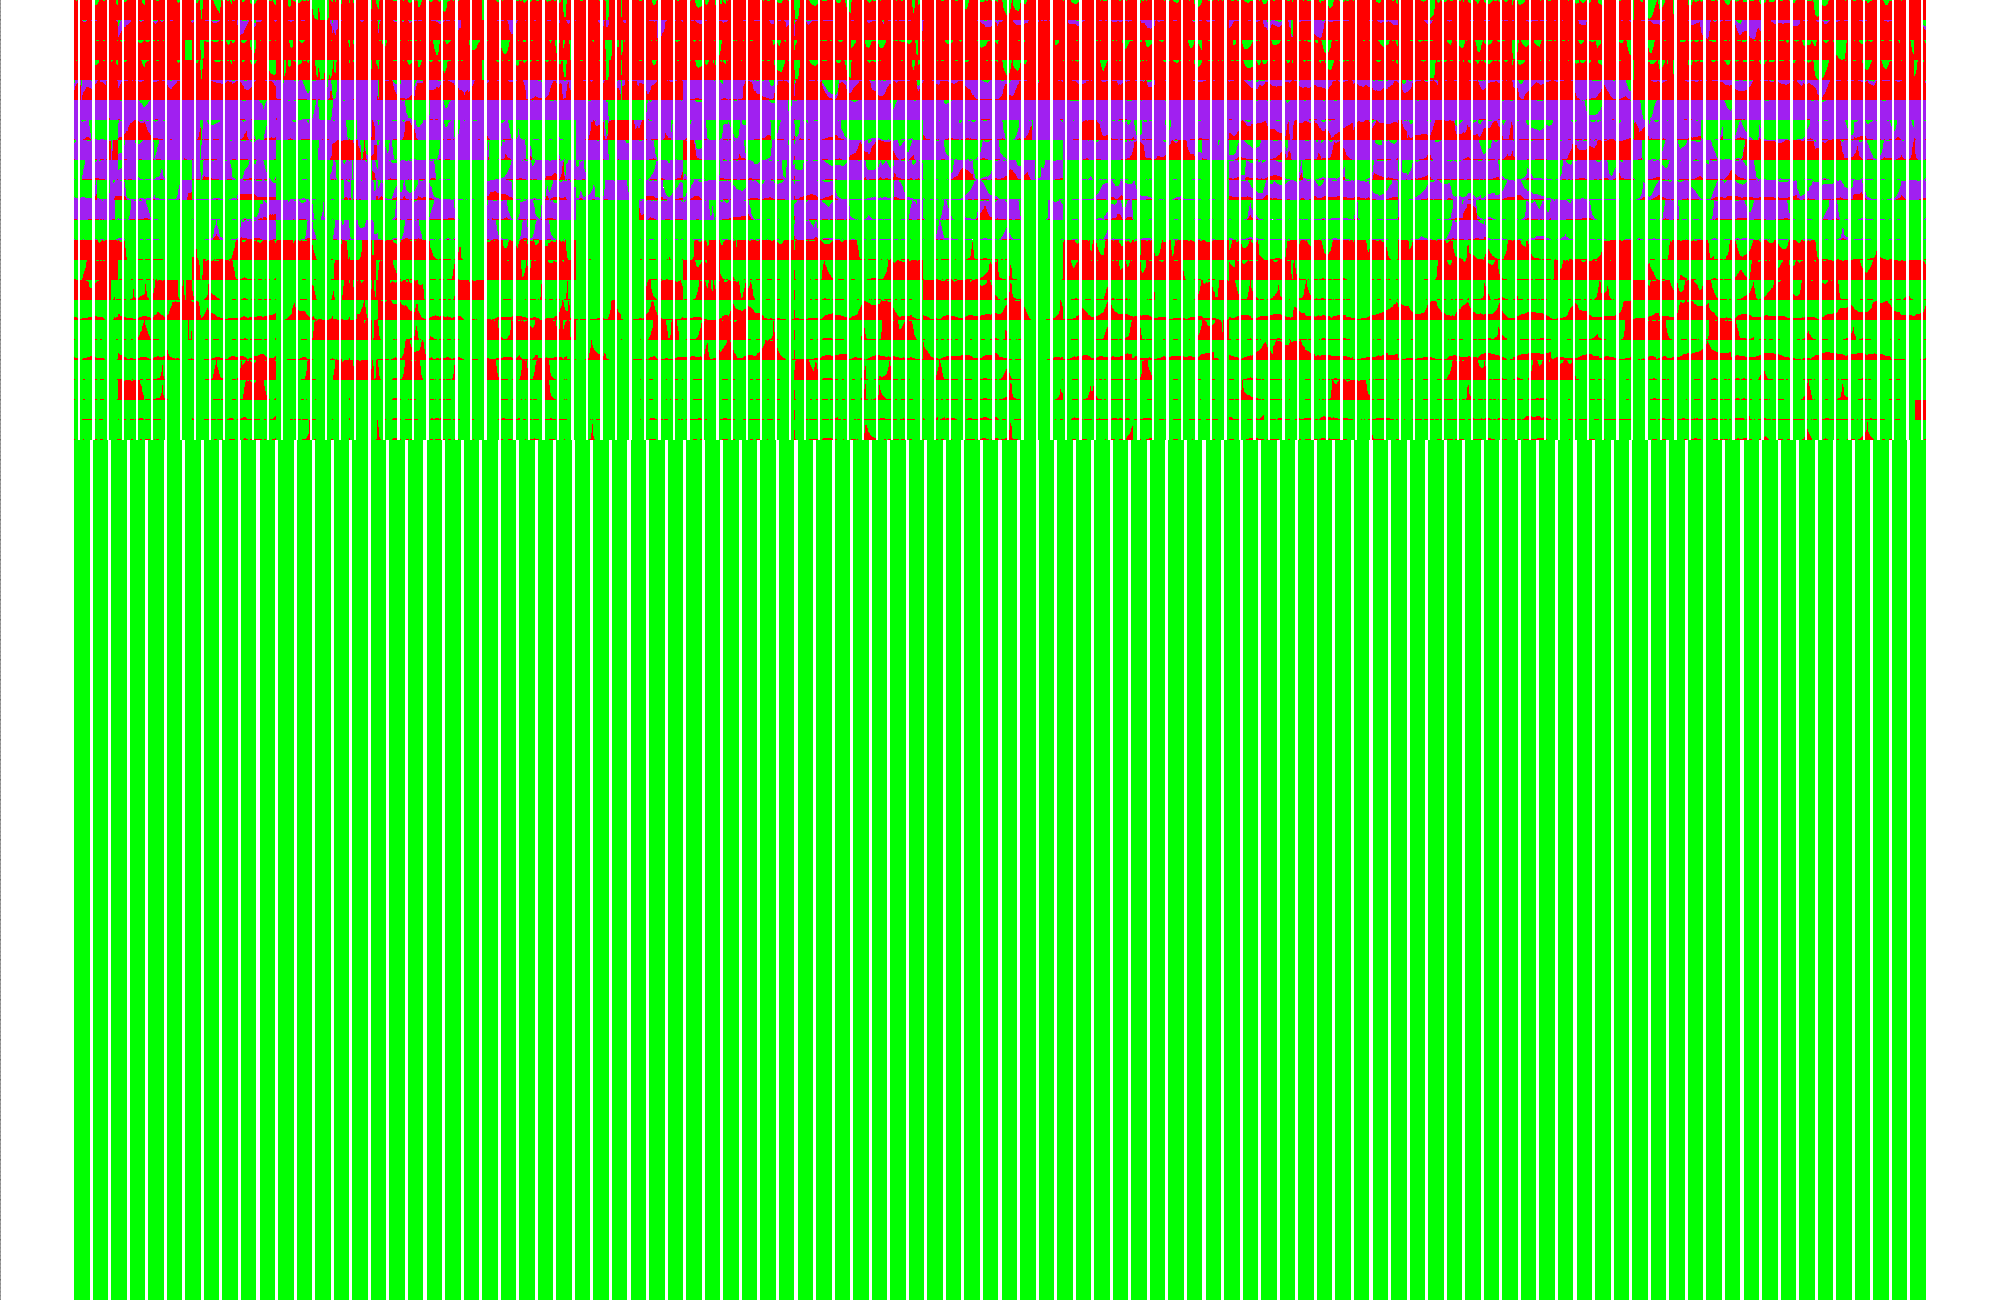
\includegraphics[width = 0.8\textwidth]{GambiaIBD.png}
  }\\
  \subfloat[][]{
  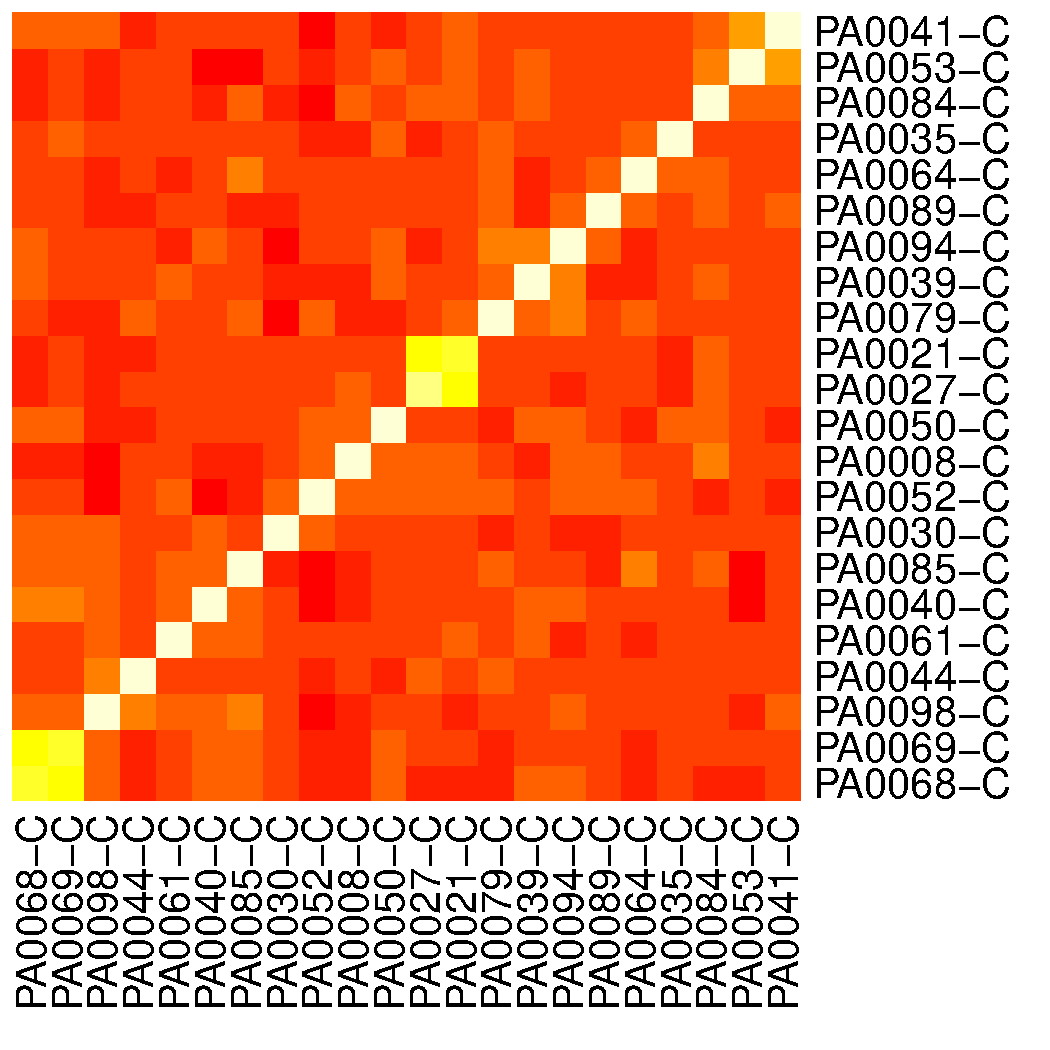
\includegraphics[width = 0.65\textwidth]{gambia_tmp.pdf}
  }\\
  \caption{(a) IBD fractions across genome of Gambia samples. Red purple and green colors indicate the fraction of the genomes are IBD. (b) Pairwise correlations of IBD fractions between mixed Gambia samples. The two yellow squares highlight two pairs of samples: PA0068-C and PA0069-C, PA0021-C and PA0027-C that share similar IBD configurations.}\label{fig:gambia}
\end{figure}


\end{document}
